% Volume I: Mathematical Language and Finite-Dimensional Geometry
% Continuity note for Chapter 5.
% Previous dependencies: Chapter 3's inner products, norms, angles, orthogonality, subspaces, and vector decompositions; Chapter 4's matrix-as-map viewpoint, column spaces, linear systems, rank, and least-squares residuals.
% New durable concepts: orthogonal projection as best approximation; projection matrices; residual orthogonality; least-squares regression as projection onto a design-matrix column space; normal equations; Gram matrices as inner-product summaries; positive semidefinite similarity matrices; QR decomposition; stable triangular least-squares solves.
% Forward hooks: Chapter 6 reuses projections, Gram matrices, and orthogonal bases for PCA, SVD, quadratic forms, and preferred directions; Chapter 7 reuses least-squares derivatives and matrix factorizations in matrix calculus; later chapters reuse projection geometry in regression, kernels, Gaussian conditioning, neural decoding, Fourier approximation, and representation learning.
% Notation commitments: y and b denote target vectors in observation space; S is a subspace; P_S is the orthogonal projection onto S; U and Q have orthonormal columns; A and X are design/basis matrices with column spaces in observation space; residuals are r=y-P_Sy or e=y-X\hat\beta; Gram matrices are X^\top X for column comparisons and XX^\top for row/observation comparisons.
% Figure plan: four existing ImageGen raster figures are used and referenced: projection as nearest point for 5.1; least-squares data-space and observation-space views for 5.2; Gram matrix similarity table for 5.3; QR orthogonalization and triangular solve for 5.4.
\section{Chapter 5: Orthogonality, Projections, and Least Squares}
\label{ch:orthogonality-projections-least-squares}

Chapter 3 introduced orthogonality as a geometric relation between vectors, and Chapter 4 showed that the columns of a matrix describe all reachable outputs of a linear model. This chapter puts those two ideas together. When a target vector is not exactly reachable, the best reachable substitute is found by projection. Least-squares regression is projection onto the column space of a design matrix. Gram matrices record the inner products that make these projections computable. QR decomposition turns a difficult correlated basis into an orthonormal one so that fitting is stable.

The unifying picture is simple: a model chooses a subspace of possible predictions, data supply a target vector, and orthogonality tells us where the closest prediction must lie.

\paragraph{Chapter problem.}
How do we replace an unreachable target by the best reachable vector, compute that replacement from data, and do so stably when the available directions are correlated?

\paragraph{Section map.}
Section 5.1 proves that projection is the nearest-point operation onto a subspace. Section 5.2 turns that theorem into least-squares regression and the normal equations. Section 5.3 studies the Gram matrices that summarize lengths, angles, similarities, and feature collinearity. Section 5.4 replaces unstable normal-equation computations with QR coordinates and a triangular solve.

\subsection{5.1 Projection as best approximation}

\paragraph{Motivating question.}
Given a vector \(y\) and a subspace \(S\), which vector \(p\in S\) is closest to \(y\)?

\paragraph{Beginner setup.}
A \emph{projection} replaces a vector by its best approximation inside a chosen subspace. The subspace is the set of vectors we are allowed to use; the original vector may lie outside it. The projected vector is the allowed vector with the smallest Euclidean error.

The smallest nontrivial example is projection onto a line. Let
\[
S=\operatorname{span}\{u\},
\qquad
u=\begin{bmatrix}1\\1\end{bmatrix},
\qquad
y=\begin{bmatrix}3\\1\end{bmatrix}.
\]
Every vector in \(S\) has the form \(cu\). We want the \(cu\) closest to \(y\). The correct coefficient is
\[
c=\frac{u^\top y}{u^\top u}
=\frac{4}{2}=2,
\]
so the projection is
\[
p=2u=\begin{bmatrix}2\\2\end{bmatrix}.
\]
The leftover vector is
\[
r=y-p=\begin{bmatrix}1\\-1\end{bmatrix}.
\]
It is perpendicular to the line because \(u^\top r=1-1=0\).

Projection solves the problem of limited representation. If a model can only produce vectors in \(S\), but the target is \(y\), then \(P_Sy\) is the best vector the model can represent under squared Euclidean error.

What to keep in mind: projection is not ``dropping a coordinate'' in general. It is the nearest-point operation determined by an inner product. The key diagnostic is residual orthogonality: after projection, the error \(y-p\) is perpendicular to every direction the model was allowed to use.

\begin{figure}[htbp]
\centering
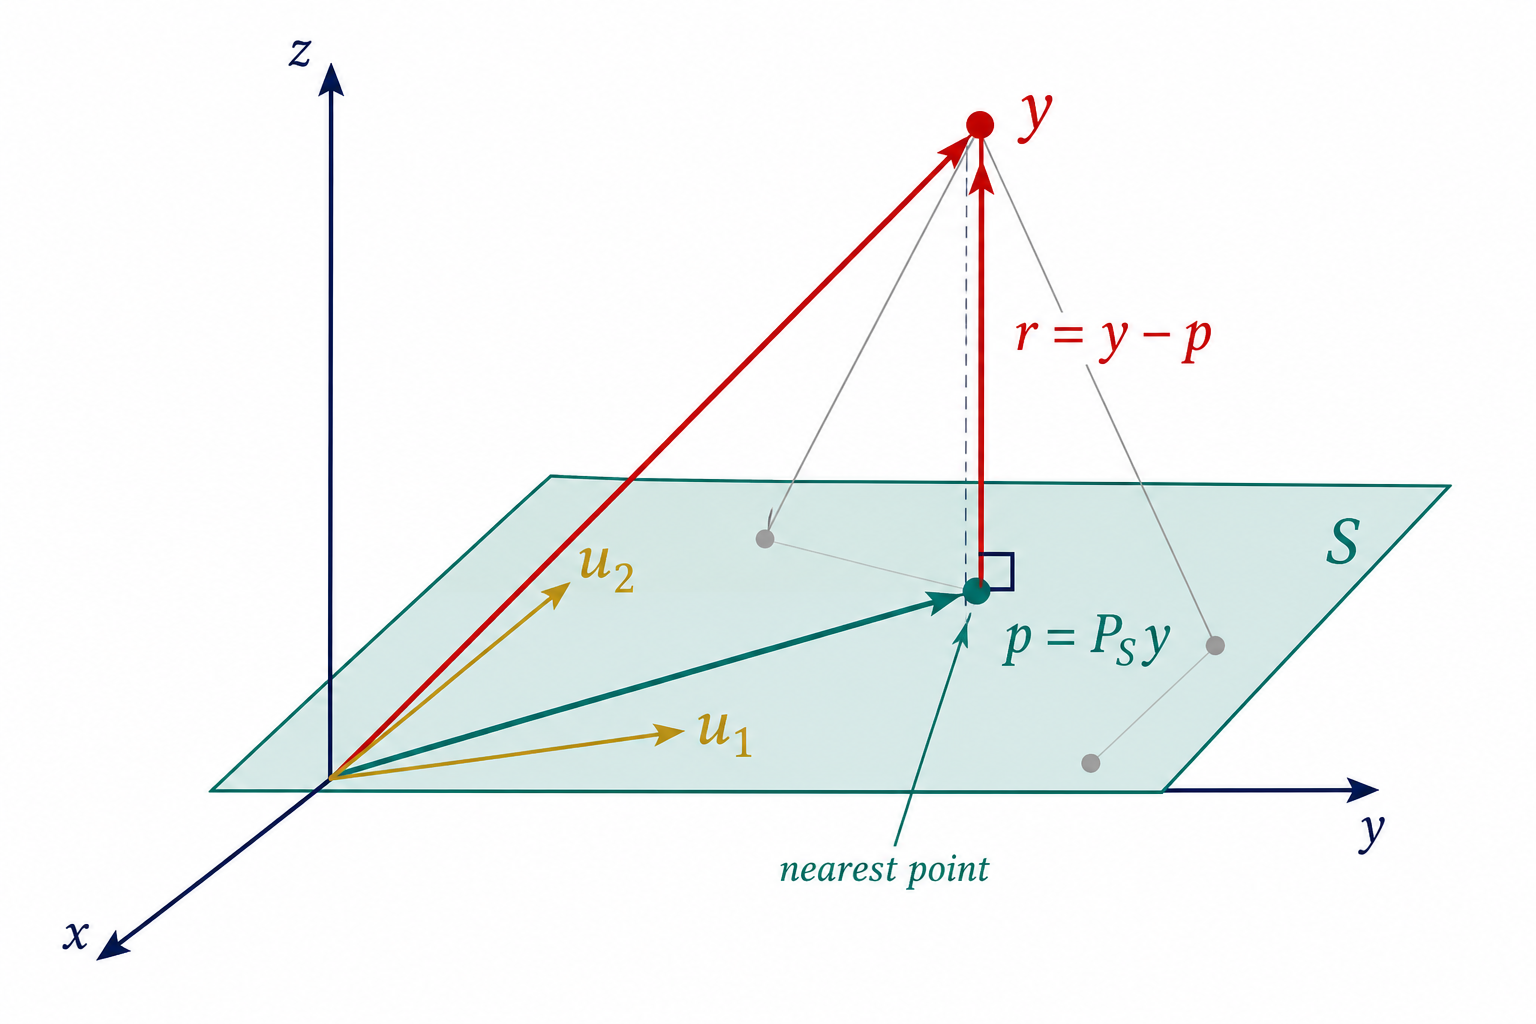
\includegraphics[width=0.95\linewidth]{imagegen-figures/ch05-projection-best-approximation.png}
\caption{Projection is a nearest-point statement. The subspace \(S\) contains all allowed approximations. The target \(y\) lies outside \(S\), so the projection \(p=P_Sy\) is the closest point in \(S\). The residual \(r=y-p\) is perpendicular to the whole subspace, not merely to the drawn basis arrows \(u_1\) and \(u_2\).}
\label{fig:ch05-projection-best-approximation}
\end{figure}

\paragraph{Formal setup.}
Work in \(\mathbb{R}^n\) with Euclidean inner product
\[
\langle x,z\rangle=x^\top z
\]
and norm \(\|x\|=\sqrt{x^\top x}\). Let \(S\subseteq\mathbb{R}^n\) be a linear subspace. The \emph{orthogonal projection} of \(y\in\mathbb{R}^n\) onto \(S\) is the vector
\[
P_Sy=\arg\min_{s\in S}\|y-s\|^2.
\]
The domain of \(P_S\) is \(\mathbb{R}^n\), its codomain is \(S\subseteq\mathbb{R}^n\), and \(P_Sy\) is the best approximation to \(y\) among vectors in \(S\).

If \(U\in\mathbb{R}^{n\times k}\) has orthonormal columns \(u_1,\dots,u_k\) spanning \(S\), so \(U^\top U=I_k\), then
\[
P_Sy=UU^\top y
=\sum_{j=1}^k u_j(u_j^\top y).
\]
If \(A\in\mathbb{R}^{n\times k}\) has linearly independent columns spanning \(S\), but the columns are not orthonormal, then
\[
P_Sy=A(A^\top A)^{-1}A^\top y.
\]
The orthonormal formula is conceptually cleaner; the non-orthonormal formula shows how projections are computed from a general basis.

\paragraph{Core intuition.}
Figure~\ref{fig:ch05-projection-best-approximation} shows the object of study. The teal plane is \(S\). The red vector \(y\) is the target. The teal vector \(p\) is the point in the plane closest to \(y\). Any movement from \(p\) within the plane goes sideways relative to the residual \(r=y-p\), so it can only increase the distance to \(y\) by adding a perpendicular component.

The phrase ``perpendicular to the subspace'' means perpendicular to every vector in the subspace:
\[
r\perp S
\qquad\Longleftrightarrow\qquad
\langle r,s\rangle=0\text{ for all }s\in S.
\]
It is not enough for \(r\) to be perpendicular to one vector drawn in the picture. For a plane, \(r\) must be perpendicular to every direction in the plane.

Common beginner misconceptions usually come from flattening the geometry too much. First, the projection point is not found by moving vertically in the page; it is found by moving perpendicular to \(S\) under the chosen inner product. Second, projection depends on the inner product. If later we use a weighted inner product, the notion of ``closest'' changes. Third, \(P_Sy\) is a vector in the same ambient space as \(y\), not a list of coordinates unless we separately choose a basis for \(S\).

This section extends Chapter 3's norm and angle geometry and Chapter 4's column-space picture. It prepares least squares, PCA, Fourier approximation, kernel methods, and projection-based views of neural population activity.

\paragraph{Main theorem: orthogonal projection theorem.}
Let \(S\) be a finite-dimensional subspace of \(\mathbb{R}^n\). For every \(y\in\mathbb{R}^n\), there is a unique vector \(p\in S\) such that
\[
y=p+r,
\qquad
r\perp S.
\]
This vector \(p\) is the unique minimizer of \(\|y-s\|^2\) over \(s\in S\).

\emph{Proof sketch.} Choose an orthonormal basis \(u_1,\dots,u_k\) for \(S\), and define
\[
p=\sum_{j=1}^k u_j(u_j^\top y).
\]
This is a vector in \(S\) because it is a linear combination of basis vectors of \(S\). Now check the residual \(r=y-p\). For each basis vector \(u_i\),
\[
u_i^\top r
=u_i^\top y-u_i^\top\sum_{j=1}^k u_j(u_j^\top y).
\]
Because the basis is orthonormal, \(u_i^\top u_j=0\) when \(i\neq j\) and \(u_i^\top u_i=1\). The sum therefore keeps only the \(j=i\) term:
\[
u_i^\top r
=u_i^\top y-u_i^\top y=0.
\]
Since \(r\) is perpendicular to every basis direction, it is perpendicular to every vector in \(S\).

To see why \(p\) is best, take any \(s\in S\). Then
\[
y-s=(y-p)+(p-s)=r+(p-s).
\]
The vector \(p-s\) lies in \(S\), while \(r\perp S\). By the Pythagorean theorem,
\[
\|y-s\|^2=\|r\|^2+\|p-s\|^2.
\]
The second term is nonnegative and is zero only when \(s=p\). Therefore \(p\) is the unique closest vector in \(S\).

\paragraph{Worked examples.}
\emph{Small numerical example.} Project
\[
y=\begin{bmatrix}2\\3\\4\end{bmatrix}
\]
onto the plane \(S=\operatorname{span}\{e_1,e_2\}\subset\mathbb{R}^3\). The columns of
\[
U=
\begin{bmatrix}
1&0\\
0&1\\
0&0
\end{bmatrix}
\]
are orthonormal and span \(S\). Thus
\[
P_Sy=UU^\top y
=
\begin{bmatrix}
1&0&0\\
0&1&0\\
0&0&0
\end{bmatrix}
\begin{bmatrix}2\\3\\4\end{bmatrix}
=
\begin{bmatrix}2\\3\\0\end{bmatrix}.
\]
The residual is \(r=(0,0,4)^\top\), which is perpendicular to every vector \((a,b,0)^\top\in S\).

\emph{Conceptual ML/neuroscience example.} Suppose a neural population response \(y\in\mathbb{R}^{100}\) records firing rates from 100 neurons on one trial. A two-dimensional task subspace \(S\) might be spanned by one direction encoding stimulus strength and another direction encoding choice. The projection \(P_Sy\) is the component of the population response explained by those two task variables. The residual \(y-P_Sy\) is not ``noise'' automatically, but it is the activity component orthogonal to that chosen task subspace. It may contain nuisance variation, unmodeled task variables, or internally generated dynamics.

\paragraph{ML/DL/neuroscience connections.}
In supervised learning, projection appears whenever predictions are restricted to a linear model class. In representation learning, projecting an embedding onto a concept direction asks how much of the embedding lies along that concept. In attention mechanisms, dot products measure alignment before values are combined; projection geometry explains why alignment is a useful primitive. In neuroscience, projecting neural activity onto task axes, decoder axes, or principal-component subspaces separates interpretable low-dimensional structure from residual activity.

\paragraph{Exercises.}
\begin{enumerate}[label=\textbf{5.1.\arabic*.}, leftmargin=*]
\item \textbf{Mechanical.} Project \(y=(4,1)^\top\) onto the line \(S=\operatorname{span}\{(1,2)^\top\}\). Compute the projection \(p\) and residual \(r=y-p\), and verify \(r\perp S\).
\item \textbf{Proof or derivation.} Let \(U\in\mathbb{R}^{n\times k}\) have orthonormal columns. Prove that \(P=UU^\top\) satisfies \(P^2=P\) and \(P^\top=P\). Interpret these two identities geometrically.
\item \textbf{Numerical/computational.} Write pseudocode that takes an orthonormal matrix \(U\) and a vector \(y\), returns \(p=UU^\top y\), and checks that \(\|U^\top(y-p)\|\) is numerically small.
\item \textbf{Interpretation.} A neural response vector is projected onto a movement-direction subspace. What does the residual represent, and why should we avoid immediately calling it noise?
\item \textbf{Debug the misconception.} A student says, ``The projection is the point directly below \(y\) on the page.'' Explain why the correct direction is perpendicular to the subspace, not necessarily vertical in the drawing.
\end{enumerate}

\subsection{5.2 Least-squares regression}

\paragraph{Motivating question.}
When the linear system \(X\beta=y\) has no exact solution, which coefficient vector \(\beta\) gives the closest predictions \(X\beta\)?

\paragraph{Beginner setup.}
Least-squares regression is the projection idea applied to data fitting. The matrix \(X\in\mathbb{R}^{n\times p}\) is the \emph{design matrix}. Its \(n\) rows are observations, and its \(p\) columns are features or regressors. The response vector \(y\in\mathbb{R}^n\) stores the measured target values. The coefficient vector \(\beta\in\mathbb{R}^p\) turns features into predictions:
\[
\hat y=X\beta.
\]
Usually \(y\) is not exactly in the column space of \(X\), so no \(\beta\) makes \(X\beta=y\). Least squares chooses \(\hat\beta\) to minimize the squared residual length
\[
\|y-X\beta\|^2.
\]

The smallest useful regression example has an intercept and one scalar feature:
\[
X=
\begin{bmatrix}
1&0\\
1&1\\
1&2
\end{bmatrix},
\qquad
y=
\begin{bmatrix}
1\\2\\2
\end{bmatrix}.
\]
The first column allows a vertical offset, and the second column allows a slope. The model predictions are all vectors on the two-dimensional plane \(\operatorname{Col}(X)\subseteq\mathbb{R}^3\).

Least squares solves the problem of approximate linear prediction. It finds the point in \(\operatorname{Col}(X)\) closest to \(y\), then returns the coefficients that produce that point.

What to keep in mind: the regression line in a scatterplot is only one picture. Algebraically, least squares projects the response vector \(y\in\mathbb{R}^n\) onto the column space of the design matrix. The residual vector is perpendicular to every column of \(X\).

\begin{figure}[htbp]
\centering
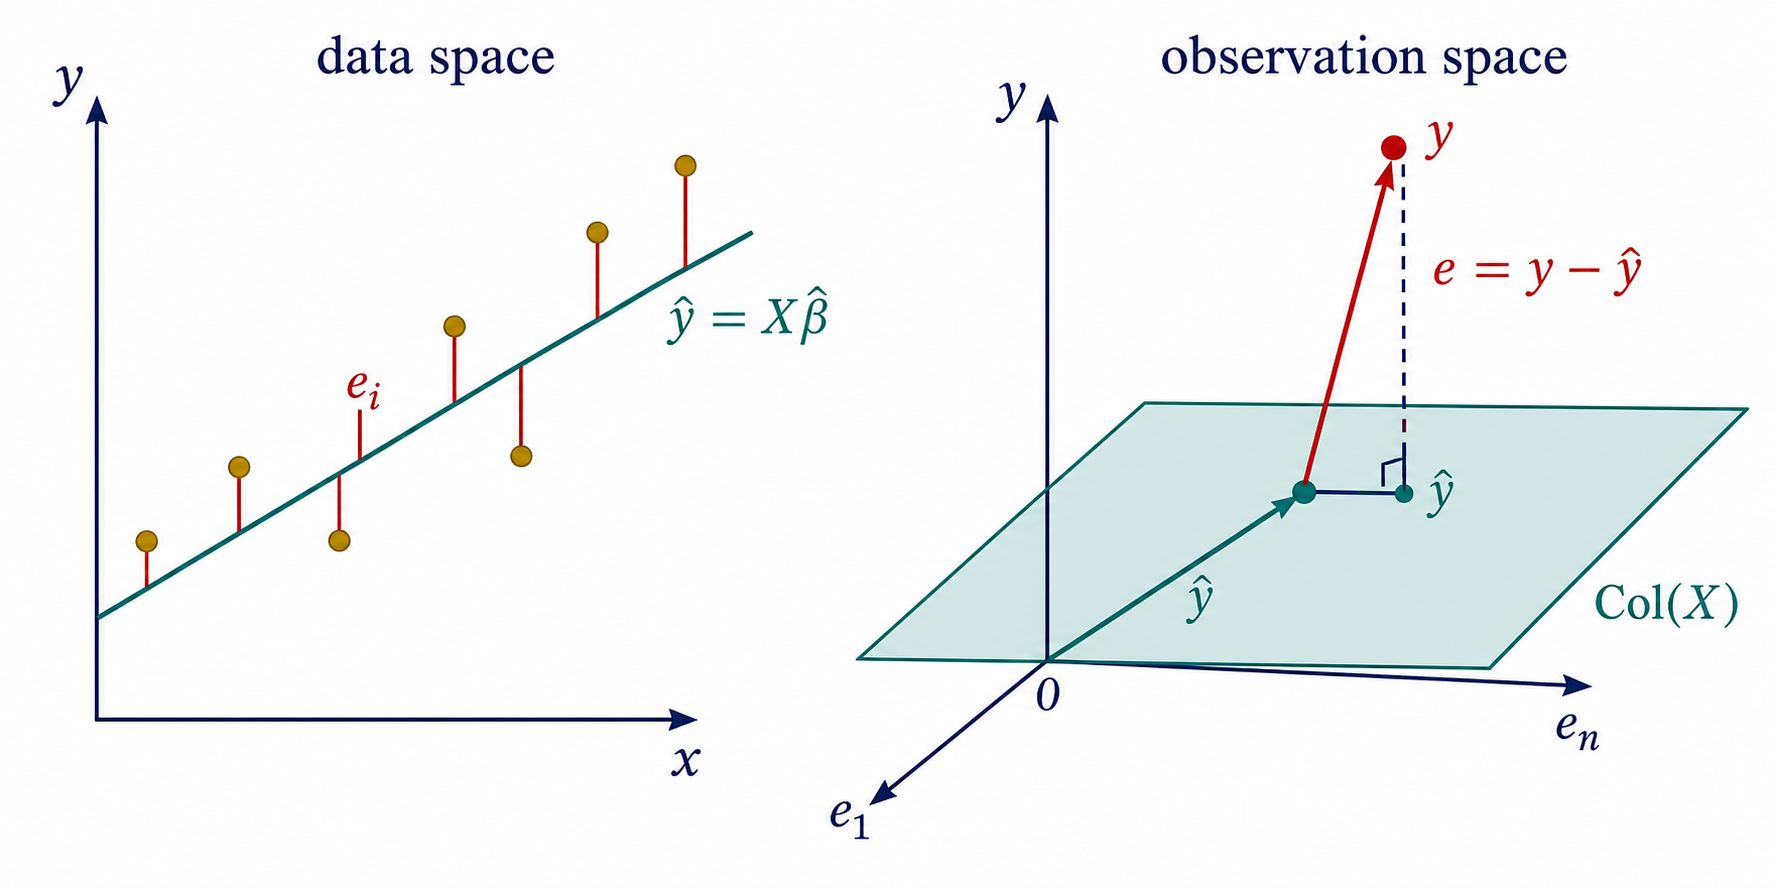
\includegraphics[width=0.95\linewidth]{imagegen-figures/ch05-least-squares-regression.png}
\caption{Least squares has two simultaneous views. In data space, residuals are vertical errors from observed responses to the fitted line. In observation space, those scalar residuals are entries of one vector \(e=y-\hat y\). The fitted vector \(\hat y=X\hat\beta\) is the projection of \(y\) onto \(\operatorname{Col}(X)\), so \(X^\top e=0\).}
\label{fig:ch05-least-squares-regression}
\end{figure}

\paragraph{Formal setup.}
Let \(X\in\mathbb{R}^{n\times p}\), \(y\in\mathbb{R}^n\), and \(\beta\in\mathbb{R}^p\). The prediction map is
\[
\beta\mapsto X\beta,
\]
whose domain is parameter space \(\mathbb{R}^p\) and whose codomain is observation space \(\mathbb{R}^n\). The set of possible predictions is \(\operatorname{Col}(X)\).

The least-squares objective is
\[
L(\beta)=\frac12\|y-X\beta\|^2
=\frac12(y-X\beta)^\top(y-X\beta).
\]
The residual is
\[
e(\beta)=y-X\beta.
\]
The normal equations are
\[
X^\top X\hat\beta=X^\top y.
\]
If \(X\) has full column rank, then \(X^\top X\) is invertible and the minimizer is unique:
\[
\hat\beta=(X^\top X)^{-1}X^\top y.
\]
If \(X\) is rank deficient, the fitted vector \(\hat y=P_{\operatorname{Col}(X)}y\) is still unique, but multiple coefficient vectors may produce the same best fitted vector. In that case the normal equations still characterize least-squares minimizers, but the inverse formula must be replaced by a rank-aware solver such as QR with pivoting, SVD, or a pseudoinverse.

The fitted vector is
\[
\hat y=X\hat\beta=P_{\operatorname{Col}(X)}y.
\]

\paragraph{Core intuition.}
Each column of \(X\) is a direction in observation space. Changing coefficient \(\beta_j\) moves the prediction along column \(x_j\). Least squares asks for the combination of columns that lands closest to \(y\). Figure~\ref{fig:ch05-least-squares-regression} shows why the residual must be orthogonal to the whole column space: if the residual had any component along a column of \(X\), we could improve the fit by moving \(\beta\) in that direction.

The common scatterplot view can hide the geometry. A line fitted through points \((t_i,y_i)\) is drawn in the \((t,y)\)-plane, but the vector \(y=(y_1,\dots,y_n)\) lives in \(\mathbb{R}^n\). The fitted vector \(\hat y=(\hat y_1,\dots,\hat y_n)\) also lives in \(\mathbb{R}^n\). The residual entries \(e_i=y_i-\hat y_i\) are coordinates of a single residual vector \(e\).

Two misconceptions are especially common. First, the best coefficients are not usually found by making residuals sum to zero only. With an intercept column, residuals do sum to zero, but least squares also requires residuals to be orthogonal to every other feature column. Second, normal equations are a mathematical characterization, not always the best numerical algorithm. Chapter 5.4 explains why QR is usually safer than explicitly solving \(X^\top X\hat\beta=X^\top y\).

This section uses the projection theorem from Section 5.1 and the column-space view from Chapter 4. It prepares linear decoders, generalized linear models, optimization, statistical estimation, and supervised learning.

\paragraph{Main derivation: normal equations from residual orthogonality.}
The least-squares minimizer \(\hat\beta\) satisfies
\[
X^\top(y-X\hat\beta)=0,
\]
equivalently
\[
X^\top X\hat\beta=X^\top y.
\]

\emph{Derivation.} Start with the objective
\[
L(\beta)=\frac12(y-X\beta)^\top(y-X\beta).
\]
Expand the quadratic:
\[
L(\beta)=\frac12 y^\top y-\beta^\top X^\top y+\frac12\beta^\top X^\top X\beta.
\]
The first term does not depend on \(\beta\). The middle term is linear in \(\beta\). The final term is quadratic and measures how prediction length changes with coefficients. Taking the gradient with respect to \(\beta\) gives
\[
\nabla_\beta L(\beta)=-X^\top y+X^\top X\beta.
\]
At a minimizer, the gradient is zero:
\[
-X^\top y+X^\top X\hat\beta=0.
\]
Rearranging gives the normal equations. In residual form,
\[
X^\top(y-X\hat\beta)=0.
\]
This says every feature column of \(X\) is orthogonal to the residual vector. Algebra and geometry are saying the same thing.

\paragraph{Worked examples.}
\emph{Small numerical example.} For
\[
X=
\begin{bmatrix}
1&0\\
1&1\\
1&2
\end{bmatrix},
\qquad
y=
\begin{bmatrix}
1\\2\\2
\end{bmatrix},
\]
we compute
\[
X^\top X=
\begin{bmatrix}
3&3\\
3&5
\end{bmatrix},
\qquad
X^\top y=
\begin{bmatrix}
5\\6
\end{bmatrix}.
\]
The normal equations give
\[
\begin{bmatrix}
3&3\\
3&5
\end{bmatrix}
\hat\beta
=
\begin{bmatrix}
5\\6
\end{bmatrix},
\qquad
\hat\beta=
\begin{bmatrix}
7/6\\
1/2
\end{bmatrix}.
\]
Thus
\[
\hat y=X\hat\beta=
\begin{bmatrix}
7/6\\
5/3\\
13/6
\end{bmatrix},
\qquad
e=y-\hat y=
\begin{bmatrix}
-1/6\\
1/3\\
-1/6
\end{bmatrix}.
\]
Check the geometry:
\[
X^\top e=
\begin{bmatrix}
1&1&1\\
0&1&2
\end{bmatrix}
\begin{bmatrix}
-1/6\\
1/3\\
-1/6
\end{bmatrix}
=
\begin{bmatrix}
0\\0
\end{bmatrix}.
\]
The residual is perpendicular to both columns of \(X\).

\emph{Conceptual ML/neuroscience example.} In a linear neural decoder, \(X\in\mathbb{R}^{n\times p}\) might contain neural activity from \(p\) neurons across \(n\) trials, and \(y\in\mathbb{R}^n\) might contain hand velocity in one direction. Least squares finds decoder weights \(\hat\beta\) so that \(X\hat\beta\) is the closest linear prediction of velocity from population activity. The residual contains the part of the velocity signal not linearly captured by the recorded neural population and chosen time window.

\paragraph{ML/DL/neuroscience connections.}
Least squares is the prototype for supervised learning. The model class is linear in parameters, the loss is squared error, and the optimum can be characterized exactly. In deep learning, the same loss appears in regression heads, distillation objectives, and local quadratic approximations to more complicated losses. In neuroscience, least squares estimates receptive fields, linear encoding models, readout weights, and trial-by-trial decoders. Later chapters generalize this picture to regularized least squares, generalized linear models, maximum likelihood, and nonlinear networks trained by gradient methods.

\paragraph{Exercises.}
\begin{enumerate}[label=\textbf{5.2.\arabic*.}, leftmargin=*]
\item \textbf{Mechanical.} Let
\[
X=\begin{bmatrix}1&0\\1&1\\1&3\end{bmatrix},
\qquad
y=\begin{bmatrix}1\\2\\4\end{bmatrix}.
\]
Compute \(X^\top X\), \(X^\top y\), and the normal equations.
\item \textbf{Proof or derivation.} Starting from \(L(\beta)=\frac12\|y-X\beta\|^2\), derive \(\nabla_\beta L=X^\top X\beta-X^\top y\) without skipping the expansion step.
\item \textbf{Numerical/computational.} Write pseudocode for fitting least squares by forming \(X^\top X\) and \(X^\top y\), solving the linear system, and reporting \(\|X^\top(y-X\hat\beta)\|\).
\item \textbf{Interpretation.} In a neural decoding problem, what does it mean if \(X^\top e=0\) but the residual norm \(\|e\|\) is still large?
\item \textbf{Debug the misconception.} A student says, ``Least squares makes every residual equal to zero.'' Explain why that is true only when \(y\in\operatorname{Col}(X)\), and state what least squares guarantees instead.
\end{enumerate}

\subsection{5.3 Gram matrices and similarity}

\paragraph{Motivating question.}
Can we understand the geometry of many vectors using only their pairwise inner products?

\paragraph{Beginner setup.}
A \emph{Gram matrix} is a table of inner products. Given vectors \(x_1,\dots,x_m\in\mathbb{R}^d\), their Gram matrix is
\[
G\in\mathbb{R}^{m\times m},
\qquad
G_{ij}=x_i^\top x_j.
\]
The diagonal entry \(G_{ii}=\|x_i\|^2\) measures the squared length of vector \(x_i\). The off-diagonal entry \(G_{ij}\) measures alignment between \(x_i\) and \(x_j\): positive if they point similarly, zero if they are orthogonal, and negative if they point in opposite directions.

A smallest nontrivial example uses three vectors in \(\mathbb{R}^2\):
\[
x_1=\begin{bmatrix}1\\0\end{bmatrix},
\qquad
x_2=\begin{bmatrix}1\\1\end{bmatrix},
\qquad
x_3=\begin{bmatrix}0\\2\end{bmatrix}.
\]
Then
\[
G=
\begin{bmatrix}
x_1^\top x_1 & x_1^\top x_2 & x_1^\top x_3\\
x_2^\top x_1 & x_2^\top x_2 & x_2^\top x_3\\
x_3^\top x_1 & x_3^\top x_2 & x_3^\top x_3
\end{bmatrix}
=
\begin{bmatrix}
1&1&0\\
1&2&2\\
0&2&4
\end{bmatrix}.
\]

Gram matrices solve the problem of representing geometry by comparisons. If distances, angles, similarities, or correlations are what matter, pairwise inner products may be more useful than the original coordinates.

What to keep in mind: a Gram matrix is not just a correlation table. It depends on the actual inner product and vector scaling. If vectors are normalized, entries become cosines. If vectors are centered and scaled, related matrices become covariance or correlation matrices.

\begin{figure}[htbp]
\centering
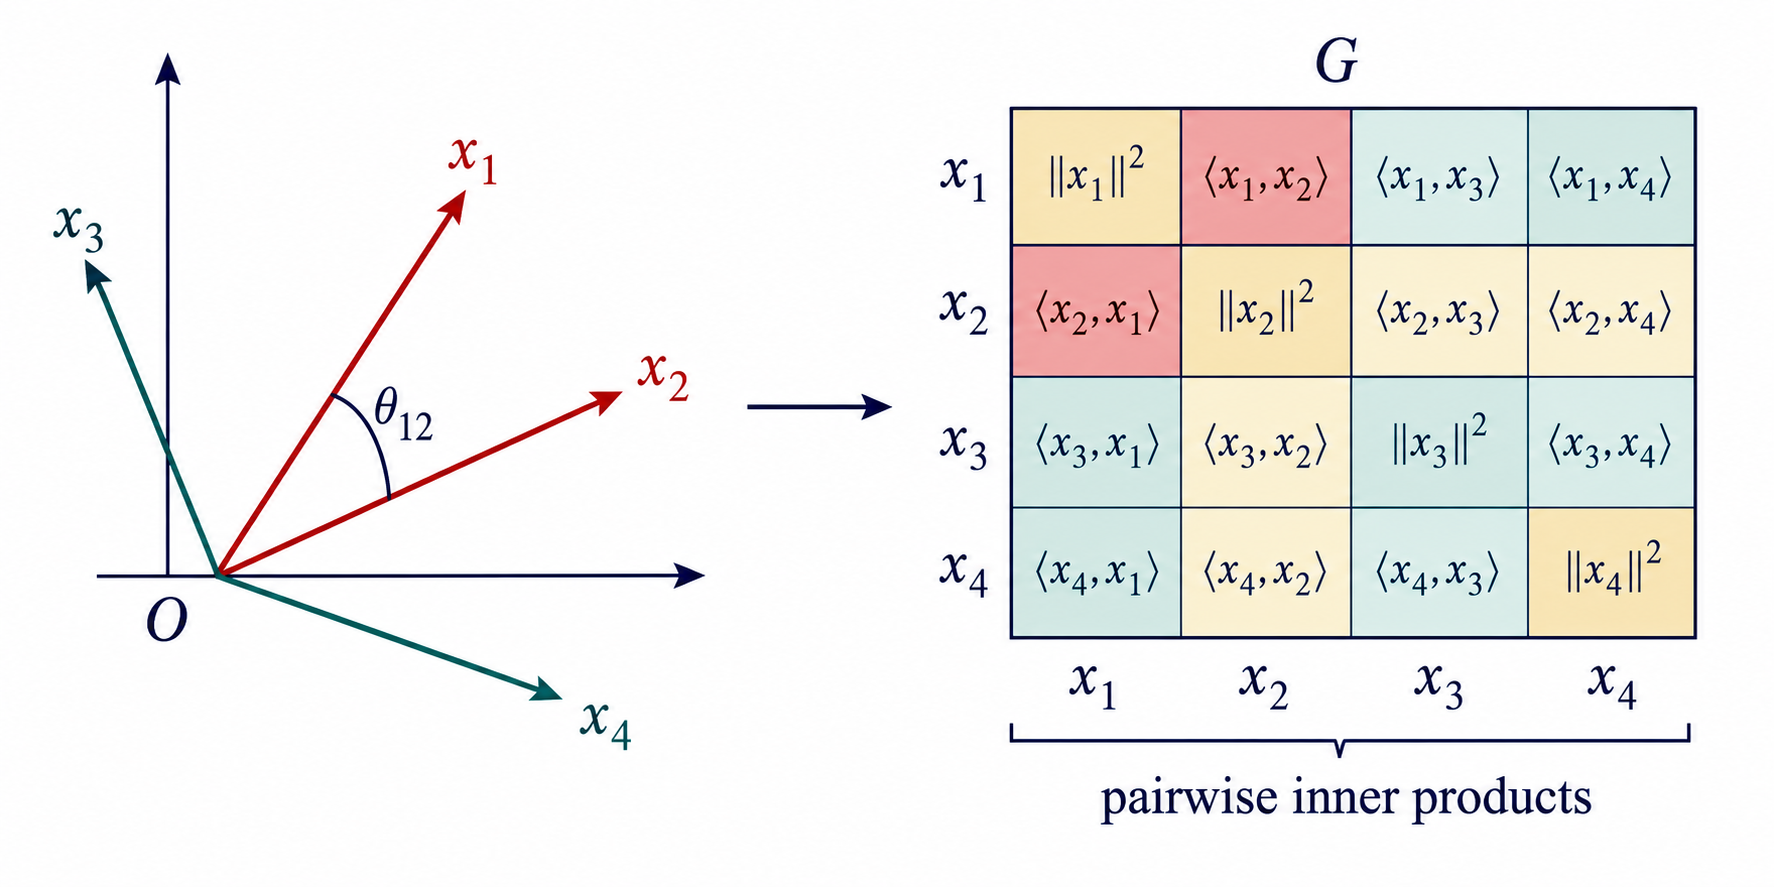
\includegraphics[width=0.95\linewidth]{imagegen-figures/ch05-gram-matrix-similarity.png}
\caption{A Gram matrix stores geometry one pair at a time. Each cell \(G_{ij}\) is the inner product \(\langle x_i,x_j\rangle\). Diagonal cells store squared lengths, while off-diagonal cells store alignment. Once \(G\) is known, distances among all vectors and angles between nonzero vectors can be recovered from these pairwise entries.}
\label{fig:ch05-gram-matrix-similarity}
\end{figure}

\paragraph{Formal setup.}
Let \(x_1,\dots,x_m\in\mathbb{R}^d\), and collect them as columns of
\[
X=\begin{bmatrix}x_1&x_2&\cdots&x_m\end{bmatrix}\in\mathbb{R}^{d\times m}.
\]
The Gram matrix is
\[
G=X^\top X\in\mathbb{R}^{m\times m},
\qquad
G_{ij}=x_i^\top x_j.
\]
It is symmetric because
\[
G_{ij}=x_i^\top x_j=x_j^\top x_i=G_{ji}.
\]
It is positive semidefinite because, for any coefficient vector \(c\in\mathbb{R}^m\),
\[
c^\top Gc=c^\top X^\top Xc=\|Xc\|^2\ge 0.
\]
If the vectors \(x_1,\dots,x_m\) are linearly independent, then \(c^\top Gc>0\) for all nonzero \(c\), so \(G\) is positive definite.

For nonzero \(x_i\) and \(x_j\), the cosine of the angle between them is
\[
\cos\theta_{ij}
=\frac{G_{ij}}{\sqrt{G_{ii}G_{jj}}}.
\]
Distances can also be recovered:
\[
\|x_i-x_j\|^2
=G_{ii}+G_{jj}-2G_{ij}.
\]

\paragraph{Core intuition.}
Figure~\ref{fig:ch05-gram-matrix-similarity} connects vectors to their comparison table. The vector drawing is geometric: length and angle are visible. The matrix drawing is computational: every length and angle is stored in entries. A large positive off-diagonal entry means two vectors share a direction strongly. A near-zero off-diagonal entry means they are nearly orthogonal. A large diagonal entry means a vector has large norm.

Beginners often confuse a Gram matrix with the original data matrix. The data matrix stores coordinates of vectors. The Gram matrix stores pairwise inner products between vectors. Another common confusion is orientation. If observations are rows in \(X\in\mathbb{R}^{n\times d}\), then \(XX^\top\in\mathbb{R}^{n\times n}\) is the observation-by-observation Gram matrix, while \(X^\top X\in\mathbb{R}^{d\times d}\) is the feature-by-feature Gram matrix. Both are Gram matrices; they compare different objects.

This section connects backward to inner products and least squares, where \(X^\top X\) appears in the normal equations. It points forward to kernels, covariance, PCA, attention scores, and representational similarity analysis.

\paragraph{Main theorem: Gram matrices encode lengths, angles, and linear independence.}
For vectors \(x_1,\dots,x_m\in\mathbb{R}^d\), the Gram matrix \(G=X^\top X\) is symmetric positive semidefinite. Its entries determine all pairwise squared distances and all angles between nonzero vectors. If \(G\) is positive definite, then the vectors are linearly independent; if the vectors are linearly independent, then \(G\) is positive definite.

\emph{Proof sketch.} Symmetry follows from the symmetry of the dot product:
\[
G_{ij}=x_i^\top x_j=x_j^\top x_i=G_{ji}.
\]
For positive semidefiniteness, choose any coefficient vector \(c\). The quadratic form of \(G\) is
\[
c^\top Gc=c^\top X^\top Xc.
\]
Regroup the products:
\[
c^\top X^\top Xc=(Xc)^\top(Xc)=\|Xc\|^2.
\]
Squared norms are always nonnegative, so \(G\) is positive semidefinite.

Distances come from expanding a squared difference:
\[
\|x_i-x_j\|^2
=(x_i-x_j)^\top(x_i-x_j)
=x_i^\top x_i+x_j^\top x_j-2x_i^\top x_j.
\]
Replace each inner product by a Gram entry to get \(G_{ii}+G_{jj}-2G_{ij}\). Angles follow from the dot-product identity \(x_i^\top x_j=\|x_i\|\,\|x_j\|\cos\theta_{ij}\).

Finally, \(G\) is positive definite exactly when \(c^\top Gc=\|Xc\|^2\) is positive for every nonzero \(c\). That fails precisely when some nonzero \(c\) satisfies \(Xc=0\), which means the columns \(x_i\) are linearly dependent.

\paragraph{Worked examples.}
\emph{Small numerical example.} For the three vectors above,
\[
G=
\begin{bmatrix}
1&1&0\\
1&2&2\\
0&2&4
\end{bmatrix}.
\]
The distance between \(x_1\) and \(x_3\) is
\[
\|x_1-x_3\|^2
=G_{11}+G_{33}-2G_{13}
=1+4-0=5.
\]
The angle between \(x_1\) and \(x_2\) satisfies
\[
\cos\theta_{12}
=\frac{G_{12}}{\sqrt{G_{11}G_{22}}}
=\frac{1}{\sqrt{2}}.
\]
So \(\theta_{12}=45^\circ\).

\emph{Conceptual ML/neuroscience example.} In a transformer attention head, queries \(q_i\) and keys \(k_j\) are learned vectors. The score matrix has entries \(q_i^\top k_j\), a cross-Gram matrix comparing every query to every key. After scaling and softmax, these similarities determine which value vectors are mixed. In neuroscience, a representational similarity matrix compares neural response patterns across stimuli. If \(x_i\) is the population response to stimulus \(i\), then \(G_{ij}=x_i^\top x_j\) measures how aligned the two population patterns are before any normalization.

\paragraph{ML/DL/neuroscience connections.}
The normal equations use the feature Gram matrix \(X^\top X\); its off-diagonal entries measure feature collinearity, which affects numerical stability and coefficient variance. Kernel methods replace \(x_i^\top x_j\) by a kernel \(k(x_i,x_j)\), allowing algorithms to work through a Gram-like matrix without explicit high-dimensional features. In deep learning, attention scores are similarity matrices built from inner products. In neuroscience, covariance and representational similarity matrices summarize neural population geometry: entries compare neurons, stimuli, time bins, or latent states depending on how the data matrix is oriented.

\paragraph{Exercises.}
\begin{enumerate}[label=\textbf{5.3.\arabic*.}, leftmargin=*]
\item \textbf{Mechanical.} Compute the Gram matrix for \(x_1=(1,2)^\top\), \(x_2=(2,0)^\top\), and \(x_3=(-1,1)^\top\).
\item \textbf{Proof or derivation.} Prove that if every pair of nonzero vectors \(x_i,x_j\) is orthogonal for \(i\neq j\), then the Gram matrix is diagonal. What are the diagonal entries?
\item \textbf{Numerical/computational.} Suppose observations are rows of \(X\in\mathbb{R}^{n\times d}\). Write pseudocode to compute both \(XX^\top\) and \(X^\top X\). State what each matrix compares.
\item \textbf{Interpretation.} In a neural representational similarity matrix with stimuli as rows, what does a large off-diagonal entry \(G_{ij}\) mean? How would normalizing each response vector change the interpretation?
\item \textbf{Debug the misconception.} A student says, ``The Gram matrix has the same information as the data matrix.'' Explain what information is preserved, what is lost, and why rotations of all vectors leave the Gram matrix unchanged.
\end{enumerate}

\subsection{5.4 QR decomposition and stable fitting}

\paragraph{Motivating question.}
How can we solve least-squares problems without making correlated columns even harder to handle by forming \(X^\top X\)?

\paragraph{Beginner setup.}
QR decomposition rewrites a matrix with correlated columns as
\[
A=QR.
\]
Here \(Q\) has orthonormal columns, and \(R\) is upper triangular. The columns of \(Q\) give a clean perpendicular coordinate system for the column space of \(A\). The matrix \(R\) records how the original columns of \(A\) are assembled from those orthonormal directions.

The smallest meaningful case has two non-orthogonal columns \(a_1,a_2\in\mathbb{R}^m\). Gram-Schmidt first normalizes \(a_1\):
\[
q_1=\frac{a_1}{\|a_1\|}.
\]
Then it removes from \(a_2\) the part already explained by \(q_1\):
\[
u_2=a_2-q_1(q_1^\top a_2),
\qquad
q_2=\frac{u_2}{\|u_2\|}.
\]
Now \(q_1\perp q_2\), and \(a_1,a_2\) can be represented using the orthonormal basis \(q_1,q_2\).

QR solves the computational problem created by non-orthogonal features. Normal equations use \(A^\top A\), which squares condition numbers and can amplify numerical error. QR keeps the projection geometry but avoids explicitly forming \(A^\top A\).

What to keep in mind: QR does not change the column space. It changes the basis used to describe that column space. The model can still make the same predictions, but the computations become more stable.

\begin{figure}[htbp]
\centering
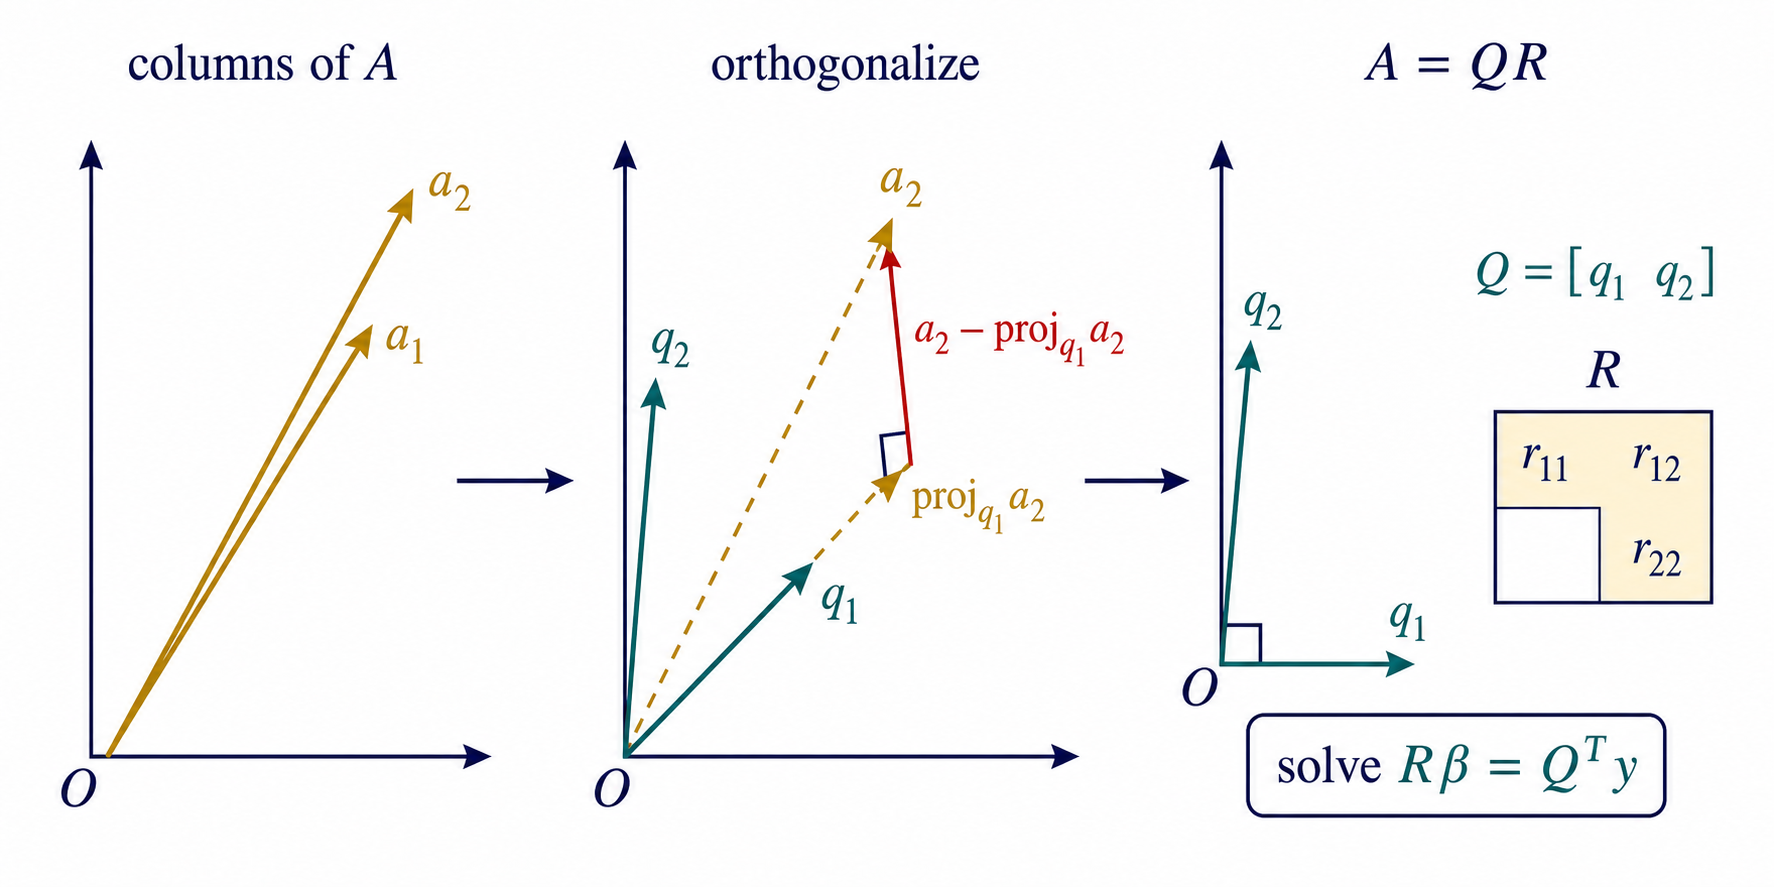
\includegraphics[width=0.95\linewidth]{imagegen-figures/ch05-qr-stable-fitting.png}
\caption{QR decomposition replaces correlated columns by orthonormal directions. The original columns \(a_1,a_2\) span the same space as \(q_1,q_2\), but the \(q\)-directions are perpendicular and unit length. The triangular matrix \(R\) records the coordinates of the original columns in the \(Q\)-basis, so least squares becomes the triangular solve \(R\hat\beta=Q^\top y\).}
\label{fig:ch05-qr-stable-fitting}
\end{figure}

\paragraph{Formal setup.}
Let \(A\in\mathbb{R}^{m\times n}\) with \(m\ge n\) and full column rank. A thin QR decomposition is
\[
A=QR,
\]
where
\[
Q\in\mathbb{R}^{m\times n},
\qquad
Q^\top Q=I_n,
\qquad
R\in\mathbb{R}^{n\times n}
\]
is upper triangular with positive diagonal entries.

For least squares,
\[
\hat\beta=\arg\min_{\beta\in\mathbb{R}^n}\|y-A\beta\|^2.
\]
Substitute \(A=QR\):
\[
\|y-A\beta\|^2=\|y-QR\beta\|^2.
\]
Because \(Q\) has orthonormal columns, the best fitted vector in \(\operatorname{Col}(A)=\operatorname{Col}(Q)\) has \(Q\)-coordinates \(Q^\top y\). Therefore the least-squares coefficients satisfy
\[
R\hat\beta=Q^\top y.
\]
Since \(R\) is triangular, \(\hat\beta\) is found by back substitution.

\paragraph{Core intuition.}
Correlated columns make coordinates fragile. If two columns point in nearly the same direction, a small change in the data can be explained by a large positive change in one coefficient and a large negative change in the other. QR separates the geometric subspace from the coordinate bookkeeping. The \(Q\) matrix gives the subspace in well-behaved perpendicular axes. The \(R\) matrix tells how to translate coefficients in the original columns into coefficients in those perpendicular axes.

Figure~\ref{fig:ch05-qr-stable-fitting} shows the mechanism. The left panel has two nearly aligned columns. The middle panel subtracts from \(a_2\) its projection onto \(q_1\), leaving a perpendicular component. The right panel keeps the clean basis \(Q=[q_1\ q_2]\) and stores the original column coordinates in \(R\).

A common misconception is that QR is a different model from least squares. It is not. It gives the same least-squares fitted vector as the projection formula, but it reaches that vector with a more stable computation. Another misconception is that Gram-Schmidt is the only QR algorithm. Classical Gram-Schmidt is a useful teaching derivation, but numerical libraries often use modified Gram-Schmidt, Householder reflections, or Givens rotations for better stability.

This section uses projections and Gram matrices from earlier in the chapter. It prepares numerical linear algebra, ridge regression, SVD, PCA, and stable fitting of high-dimensional neural and machine-learning models.

\paragraph{Main theorem: QR least squares.}
Let \(A\in\mathbb{R}^{m\times n}\) have full column rank and thin QR decomposition \(A=QR\). For any \(y\in\mathbb{R}^m\), the least-squares solution of
\[
\min_\beta \|y-A\beta\|^2
\]
is the unique vector \(\hat\beta\) satisfying
\[
R\hat\beta=Q^\top y.
\]

\emph{Proof sketch.} Since \(A=QR\) and \(R\) is invertible, \(A\) and \(Q\) have the same column space. Therefore fitting \(A\beta\) is equivalent to finding the closest vector in \(\operatorname{Col}(Q)\), but with coordinates constrained through \(R\beta\).

Decompose \(y\) into its projection onto \(\operatorname{Col}(Q)\) and its orthogonal residual:
\[
y=QQ^\top y+(I-QQ^\top)y.
\]
Then
\[
y-QR\beta
=Q(Q^\top y-R\beta)+(I-QQ^\top)y.
\]
The first term lies in \(\operatorname{Col}(Q)\). The second term is orthogonal to \(\operatorname{Col}(Q)\). By Pythagoras,
\[
\|y-QR\beta\|^2
=\|Q(Q^\top y-R\beta)\|^2+\|(I-QQ^\top)y\|^2.
\]
Because \(Q^\top Q=I\), multiplying by \(Q\) preserves lengths inside \(\mathbb{R}^n\):
\[
\|Q(Q^\top y-R\beta)\|^2=\|Q^\top y-R\beta\|^2.
\]
The second term does not depend on \(\beta\), so the minimum occurs when
\[
Q^\top y-R\hat\beta=0.
\]
Thus \(R\hat\beta=Q^\top y\). Since \(R\) is invertible, the solution is unique.

\paragraph{Worked examples.}
\emph{Small numerical example.} Let
\[
A=
\begin{bmatrix}
1&1\\
1&0\\
0&1
\end{bmatrix}
=
\begin{bmatrix}
|&|\\
a_1&a_2\\
|&|
\end{bmatrix}.
\]
The first QR vector is
\[
q_1=\frac{a_1}{\|a_1\|}
=\frac{1}{\sqrt2}
\begin{bmatrix}
1\\1\\0
\end{bmatrix},
\qquad
r_{11}=\sqrt2.
\]
Next,
\[
r_{12}=q_1^\top a_2=\frac{1}{\sqrt2},
\qquad
u_2=a_2-r_{12}q_1
=
\begin{bmatrix}
1/2\\-1/2\\1
\end{bmatrix}.
\]
Thus
\[
r_{22}=\|u_2\|=\frac{\sqrt6}{2},
\qquad
q_2=\frac{u_2}{r_{22}}
=\frac{1}{\sqrt6}
\begin{bmatrix}
1\\-1\\2
\end{bmatrix}.
\]
So
\[
Q=
\begin{bmatrix}
1/\sqrt2&1/\sqrt6\\
1/\sqrt2&-1/\sqrt6\\
0&2/\sqrt6
\end{bmatrix},
\qquad
R=
\begin{bmatrix}
\sqrt2&1/\sqrt2\\
0&\sqrt6/2
\end{bmatrix}.
\]
For \(y=(2,1,0)^\top\),
\[
Q^\top y=
\begin{bmatrix}
3/\sqrt2\\
1/\sqrt6
\end{bmatrix}.
\]
Solving \(R\hat\beta=Q^\top y\) gives
\[
\hat\beta=
\begin{bmatrix}
4/3\\
1/3
\end{bmatrix}.
\]
The fitted vector is
\[
A\hat\beta=
\begin{bmatrix}
5/3\\4/3\\1/3
\end{bmatrix},
\]
and the residual \((1/3,-1/3,-1/3)^\top\) is orthogonal to both columns of \(A\).

\emph{Conceptual ML/neuroscience example.} Suppose two regressors in a neural encoding model are highly correlated: stimulus contrast and pupil-linked arousal may rise together across trials. The columns of \(X\) are then nearly aligned. Normal equations form \(X^\top X\), where this near-alignment becomes a nearly singular Gram matrix. QR instead builds orthonormal trial-space directions \(Q\) and solves a triangular system. The fitted predictions are the same least-squares predictions, but the computation is less sensitive to roundoff and collinearity.

\paragraph{ML/DL/neuroscience connections.}
QR is a numerical foundation for stable linear regression, online orthogonalization, and basis construction. In machine learning pipelines, it appears in least-squares solvers, feature preprocessing, randomized linear algebra, and low-rank methods. In deep learning, orthogonalization ideas appear in initialization, normalization, and subspace methods for analyzing representations. In computational neuroscience, QR helps fit encoding and decoding models when regressors, neurons, or basis functions are strongly correlated.

\paragraph{Exercises.}
\begin{enumerate}[label=\textbf{5.4.\arabic*.}, leftmargin=*]
\item \textbf{Mechanical.} Apply Gram-Schmidt to \(a_1=(1,0,1)^\top\) and \(a_2=(1,1,0)^\top\). Compute \(q_1,q_2,r_{11},r_{12},r_{22}\).
\item \textbf{Proof or derivation.} Prove that if \(A=QR\) with \(Q^\top Q=I\) and invertible \(R\), then \(\operatorname{Col}(A)=\operatorname{Col}(Q)\).
\item \textbf{Numerical/computational.} Write pseudocode for solving least squares from a QR factorization: compute \(b=Q^\top y\), solve \(R\hat\beta=b\) by back substitution, then compute the residual norm.
\item \textbf{Interpretation.} In a design matrix with two nearly identical feature columns, why can coefficient estimates be unstable even when the fitted predictions are accurate? How does QR help the computation?
\item \textbf{Debug the misconception.} A student says, ``QR changes the regression problem because \(Q\) has different columns than \(A\).'' Explain why the fitted subspace is unchanged and what role \(R\) plays.
\end{enumerate}

The chapter's durable lesson is approximation geometry: when the target is outside the model's reachable set, the best linear prediction is the projection, and the residual is forced into an orthogonal complement. Least squares is this geometry with a design matrix; Gram matrices are the inner-product summaries that reveal similarity and collinearity; QR is the stable coordinate system that computes the same fit without unnecessarily worsening conditioning.

Chapter 6 reuses these ideas immediately. PCA asks for projection subspaces that preserve as much variance as possible. SVD builds orthonormal input and output directions for general matrices. Quadratic forms and covariance matrices are Gram-like objects whose preferred directions are eigenvectors. Later, the same projection picture will reappear in kernel regression, Bayesian Gaussian conditioning, Fourier approximation, neural population decoding, and low-dimensional representation analysis.

\clearpage
